\documentclass{csustThesis}
\addbibresource[location=local]{reference.bib}

% 填写基本信息、包括封面、扉页、诚信声明、摘要、开题报告封面、外文译文及原文封面和任务书封面的信息。

%%%%%%%%%%%%%%%%%%%%%%%%%%%%%%%%%%%%%%%%%%%%%%%%%% 通用基本信息 %%%%%%%%%%%%%%%%%%%%%%%%%%%%%%%%%%%%%%%%%%%%%%%%%%
\thesisTitle
{基于 \LaTeX 系统的长沙理工大学\\本科生毕业论文模板}  % 论文题目,使用\\断行
{A CSUST Bachelor thesis template\\based on \LaTeX{} system} % 论文英文题目,英文摘要用

\thesisCompleteTime{\the\year}{\the\month}{9} % 论文完成时间,依次填写年、月、日
% \singleLineTitle  % “题目”一栏默认显示两条横线,若要隐藏第二条横线,请取消该行注释。

\stuName{XXX} % 学生姓名

\stuID{2018xxxxyyyy} % 学号

\stuClass
{软件18-x班} % 班级
{18-x}  % 班级号,任务书封面用

\stuMajor{软件工程} % 专业

\supervisorName{xxx} % 指导教师姓名

\stuCollege
{计算机与通信工程学院} % 学生所在学院
{计算机与通信工程} % 学生所在学院不写学院,任务书封面用

%%%%%%%%%%%%%%%%%%%%%%%%%%%%%%%%%%%%%%%%%%%%%%%%%% 诚信声明专属信息 %%%%%%%%%%%%%%%%%%%%%%%%%%%%%%%%%%%%%%%%%%%%%%%%%%
\integrityStatementAuthor{} % 诚信声明作者签名,默认手写
\integrityStatementDate{}{}{} % 诚信声明年月日,默认手写

%%%%%%%%%%%%%%%%%%%%%%%%%%%%%%%%%%%%%%%%%%%%%%%%%% 任务书封面专属信息 %%%%%%%%%%%%%%%%%%%%%%%%%%%%%%%%%%%%%%%%%%%%%%%%%%
\taskRangeTime{\the\year 年??月??日~\the\year 年??月??日}  % 任务起止日期
% 由于任务书的指导教师、教研室主任和院长栏目需要手写签名,因此本模板暂不提供接口
% 如需更改请找到 csustThesis.cls 文件中 \makeTaskBookCover 命令,在相应位置嵌入文字即可

%%%%%%%%%%%%%%%%%%%%%%%%%%%%%%%%%%%%%%%%%%%%%%%%%% 摘要专属信息 %%%%%%%%%%%%%%%%%%%%%%%%%%%%%%%%%%%%%%%%%%%%%%%%%%
% \abstractZhtitle{基于 \LaTeX 系统的长沙理工大学本科生毕业论文模板}  % 中文摘要题目,默认为论文题目,取消注释即可更改
% \abstractEntitle{A CSUST Bachelor thesis template\\based on \LaTeX{} system}  % 默认为论文英文题目,取消注释即可更改


%%%%%%%%%%%%%%%%%%%%%%%%%%%%%%%%%%%%%%%%%%%%%%%%%% 外文译文及原文封面专属信息 %%%%%%%%%%%%%%%%%%%%%%%%%%%%%%%%%%%%%%%%%%%%%%%%%%
\researchProposalDate{\the\year}{3}  % 开题报告封面日期,依次填写年、月


%%%%%%%%%%%%%%%%%%%%%%%%%%%%%%%%%%%%%%%%%%%%%%%%%% 外文译文及原文封面专属信息 %%%%%%%%%%%%%%%%%%%%%%%%%%%%%%%%%%%%%%%%%%%%%%%%%%
\translationDate{\the\year}{3}  % 外文译文及原文封面日期,依次填写年、月
\translationRef{Adams P. The title of the work[J]. The name of the journal, 1993, 4(2): 201-213.}  % 外文译文出处,可自行调整参考文献格式


\begin{document}

\makecover % 制作封面

\maketitle % 制作扉页

\makeIntegrityStatement % 制作诚信声明

% \includepdf[pages=-]{任务书.pdf}



%% 摘要开始需要页眉,已在文档类 csustThesis 中设置 %%

\begin{abstract}

% 前面记得空一行
清华北大、复旦上交等众多国内知名大学早已拥有自己的 \LaTeX 模板,而长沙理工大学至今(2022年6月)无人发起与维护。今日某长理 18 级学子决定制作一份简陋的长沙理工大学本科生毕业论文 \LaTeX
模板,权当抛砖引玉。

% 前面记得空一行
\keywords{关键词:} 长沙理工大学;本科生毕业论文模板;\LaTeX 系统
% 第一个关键词:所属二级学科名
% 第二个关键词:研究所得成果名
% 第三个关键词:研究方法具体名称
% 第四个关键词:前三个中未出现、但作为主要研究对象的事物名称
% 第五个关键词:有利于检索和文献利用的其他关键词
\end{abstract}

\begin{abstract*}
  
% Remember to leave a blank line
Many well-known domestic universities such as Tsinghua University, Peking University, Fudan University and Shanghai Jiaotong University already have their own \LaTeX{} templates, but Changsha University of Science and Technology has not issued and maintained so far (June 2022). Today, a common sense 18th grade student decided to make a simple undergraduate graduation thesis of Changsha University of Science and Technology \LaTeX
Template, right when throwing a brick to attract jade.
  
% Remember to leave a blank line
\keywords*{Key words: } CSUST; Bachelor thesis template; \LaTeX{} system
\end{abstract*}










% BO 编译器是一个能 将高级语言源程序转化为可由 BOVM 虚拟机直接执行的字节码
%     本文呈现了 BO 编译器的设计与实现


% 随着编译理论的不断发展和各种自动化工具的出现,设计并实现一个满足特定需求的编译器变得越来越容易,各式各样的编程语言也因此不断涌现。本文介绍了如何借助 Flex 与 Bison 等自动化工具、使用 C++ 语言实现。在本文中,我们

    
% 随着编译技术的不断发展和各种自动化工具的出现,编译器的设计和开发工作越来越规范化,众多编程语言也因此不断涌现。然而当下还没有任何一种语言能够满足。设计并实现一个满足特定需求的编译器也因此变得越来越容易。

% 随着编译技术的不断发展和各种自动化工具的出现,编译器的设计和开发过程越来越规范化,设计并实现一个满足特定需求的编译器也因此变得越来越容易。在本文中,我们设计并借助 Flex 与 Bison 工具、使用 C++ 语言实现了 BO 编译器 定义了能被 BO 编译器正确识别并转化为字节码的高级语言称为 BO 语言,并使用扩展 BNF 范式描述了这种语言。实现了 BO 编译器。
% 我们使用 EBNF 范式描述 BO 编译器能够识别的 
% 人们可以在短时间内规范地设计并实现自己需要的编译器。在本文中,我们借助 Flex 与 Bison 生成 BO 编译器的 定义了能被 BO 编译器正确识别并转化为字节码的高级语言称为 BO 语言。 
% 我们将能被 BO 编译器正确识别并转化为字节码的高级语言称为 BO 语言。本文将展示如何借助 Flex 与 Bison 

% BO(Binary Object)语言是一种支持面向对象的程序设计语言,本课题将从词法分析、语法分析、中间代码生成、以及一些简单的编译优化的角度详细介绍并实现 BO 语言编译器。  % 摘要

\makecontents  % 目录

%% 正文开始加上页脚
\fancyfoot[C]{\zihao{-5} 第 \thepage 页,共 \pageref{LastPage} 页}  % 设置页脚中心
\pagenumbering{arabic}  % 页脚采用阿拉伯数字编号
%%

\chap{绪论}

\sect{研究背景}
长沙理工大学教务处官网上的\href{https://www.csust.edu.cn/jwc/sjjx/bysj.htm}{毕业设计word模板}\footnote{本文撰写时(2022年6月),官网的毕设模板发布时间为2020年10月。若今后官网更新了模板,本节仅供参考。}存在许多值得诟病的地方。


\sect{国内外研究现状}
清华北大、复旦上交等众多国内知名大学早已拥有自己的 \LaTeX 模板,而长沙理工大学至今(2022年6月)无人发起与维护。

\sect{研究意义}
该研究会使长沙理工大学也拥有一份非官方的 \LaTeX ,可以为今后想使用 \LaTeX 撰写毕业论文的学弟学妹带来方便。

\sect{论文结构}

\vspace{-1.5\baselineskip}
\begin{description}
    \item[\hspace{2em}]\!\!
\begin{description}
    \item[第一章] 绪论。简述本课题的研究背景、简述国内外研究现状、阐明课题研究内容及意义。
    \item[第二章] 需求分析。
    \item[第三章] 软件工具原理与优缺点。介绍设计和实现BO编译器所用到的软件工具及其原理,包括词法分析器和语法分析器的自动生成工具 Flex 和 Bison 、用于描述上下文无关文法的 BNF 范式、以及跨平台的项目打包工具 Cmake 等。
    \item[第四章] 总体设计。设计 BO 编译器各模块的接口及功能,介绍 BO 语言的特性及运行过程,简述 BOVM 虚拟机的工作方式。
    \item[第五章] 详细设计与系统实现。详细介绍 BO 编译器各阶段基本功能的实现以及 BO 编译器对部分 BO 语言特性的实现。
    \item[第六章] 测试。通过对BO编译器进行系统化测试找出编译器存在的潜在问题、检验编译器的质量。
\end{description} 
\end{description}  % 第1章 绪论

\chap{\LaTeX 简介}
\label{chap_tools}  % 供后文引用
  % 第2章 LaTeX 简介


\chap{模板设计与实现}
本模板遵循2020年10月发布的\href{https://www.csust.edu.cn/jwc/info/1142/3568.htm}{《长沙理工大学本科毕业设计撰写规范》}(以下简称《撰写规范》)。本文于2022年6月撰写,若今后学校模板发生变化,请自行更改模板。

\sect{目录结构}

\sect{论文模板全局设置}
本模板的大部分设置都已封装在 csustThesis 文档类中,该文档类的内容可在文件 csustThesis.cls 中找到。 csustThesis 文档类基于 article 基本文档类和 ctex 宏包实现。

\subsect{字体字号设置}

本模板中文字体采用 Windows 系统自带的宋体、黑体\footnote{使用其他操作系统的用户请自行安装相应字体或者更改模板设置。}。中文字体默认采用宋体,西文字体默认采用 Times New Roman 。
\begin{lstlisting}[numbers=none,language=TeX]
% 默认字体设置
\setCJKmainfont{宋体}[AutoFakeBold={2.17}]  % 中文默认使用 Windows 系统自带的宋体
\setmainfont{Times New Roman}  % 西文默认使用 Times New Roman
% 使用 Windows 系统自带的黑体
\setCJKfamilyfont{SimHei}[AutoFakeBold={2.17}]{黑体}
\def\heiti{\CJKfamily{SimHei}}
\end{lstlisting}

正文字号为小四、1.5倍行距,在引入 ctex 宏包时配置选项。
\begin{lstlisting}[numbers=none,language=TeX]
\RequirePackage[zihao=-4,heading=true,linespread=1.5]{ctex}
\end{lstlisting}

\subsect{页面布局设置}

本模板页面采用 A4 大小编排,并设置 上边距 25mm、下边距 20mm、左边距 30mm、右边距 20mm。
\begin{lstlisting}[numbers=none,language=TeX]
\RequirePackage[a4paper,top=25mm,bottom=20mm,left=30mm,right=20mm]{geometry}
\end{lstlisting}

设置页面页眉左侧为 \fbox{
\includegraphics[height=1.15cm]{figure/template/csust_logo_and_name2.pdf}} 、右侧为小论文标题,设置页脚中心为阿拉伯数字编号的“第几页,共几页”样式。页眉页脚文字均为小五号宋体。出于方便考虑,页脚的设置并没有封装在 csustThesis 文档类中。
\begin{lstlisting}[numbers=none,language=TeX]
% 页眉页脚预设置
\pagestyle{fancy}
\fancyhf{}

% 页眉设置
\fancyhead[L]{  % 设置页眉左侧
    \raisebox{-.1cm}{
\includegraphics[height=1.15cm]{figure/template/csust_logo_and_name2.pdf}}
}
\fancyhead[R]{\let\\=\relax\heiti\zihao{-5}\csustThesis@title}  % 设置页眉右侧

%% 正文开始加上页脚
\fancyfoot[C]{\zihao{-5} 第 \thepage 页,共 \pageref{LastPage} 页}  % 设置页脚中中心
\pagenumbering{arabic}  % 页脚采用阿拉伯数字编号
%%
\end{lstlisting}

\subsect{标题设置}
本模板支持三级标题,一级标题样式为黑体小三居中,使用命令 \verb!\chap! 定义;二级标题样式为黑体四号顶格,使用命令 \verb!\sect! 定义;三级标题样式为黑体小四且缩进两字符,使用命令 \verb!\subsect! 定义。
\begin{lstlisting}[numbers=none,language=TeX]
% 标题设置
\ctexset{
	section = {  % 一级标题
		format = \centering\heiti\zihao{-3},  % 黑体小三居中
		name = {第, 章},  % 章节编号为 “第几章”
	},
	subsection = {  % 二级标题
		format = \heiti\zihao{4},  % 黑体四号
	},
	subsubsection = {  % 三级标题
		format = \heiti\zihao{-4},  % 黑体小四
        indent = 2\ccwd,  % 缩进两字符
	}
}

\newcommand{\chap}[1]{%
	\clearpage  % 每章另起一页
    \FloatBarrier  % 清除浮动体,也就是输出上一章的图表
    \vspace*{-.5\baselineskip}  % 调整章标题与页眉顶部的间距
	\section{#1}
}
\newcommand{\sect}[1]{\subsection{#1}}
\newcommand{\subsect}[1]{\subsubsection{#1}}
\end{lstlisting}

\subsect{图表名格式设置}
本模板支持图(figure)和表(table)两种浮动体,且支持图表名自动按章节编号。图题为五号字体,图序为“图几.几”格式。表题为五号\textbf{加粗}字体,表序为“表几-几”格式。

\begin{lstlisting}[numbers=none]
\captionsetup{font=small,labelsep=space}  % 图表标题设为五号字体、序号与图表名之间以空格分隔
\captionsetup[table]{font={small,bf},labelsep=space}  % 表标题设为五号加粗、表序与表名之间以空格分隔
\counterwithin{figure}{section}  % 图按章节编号
\counterwithin{table}{section}  % 表按章节编号
\renewcommand{\thefigure}{\thesection.\arabic{figure}}  % 图几.几
\renewcommand{\thetable}{\thesection-\arabic{table}}  % 表几-几
\end{lstlisting}

\subsect{代码抄录环境设置}
本模板的代码抄录使用 listings 宏包的 \verb!lstlisting! 环境、通过 \verb!\lstset! 进行全局设置。默认白色背景、有边框、有行号等等。

\subsect{参考文献样式设置}
本模板使用 biblatex 宏包进行参考文献自动管理,采用 GB7714-2015 样式。虽然论文撰写规范中明确表示参考文献著录应符合 GB7714-87 标准,但是撰写规范样张给出的示例都更接近 GB7714-2015 样式。若要使用 GB7714-1987 样式,需要 texlive 2022 或更新的版本。

\subsect{附录设置}
本模板重写了基本文档类的 \verb!\appendix! 命令。

附录与正文的区别主要有:一级标题样式变为黑体三号居中、采用大写字母编号;插图与表格的编号没有分隔符,如图A1、表B2。

官网模板的撰写规范和样张中都没有体现附录的二级标题与三级标题如何处理,因此本模板附录的二、三级标题样式\textcolor{red}{保持与正文一致,但不编入目录}。

\sect{封面与扉页的设计}
本模板的封面和扉页均参考\href{https://www.csust.edu.cn/jwc/info/1142/3596.htm}{《毕业设计(论文)封面、扉页》}设计,对应的命令分别为 \verb!\makecover! 和 \verb!\maketitle! 。

封面题目采用宋体小二加粗并居中、扉页题目采用黑体二号加粗并居中。应填写的信息均采用宋体三号加粗并居中。

\sect{摘要与目录的设计}
本模板的摘要和目录均参考\href{https://www.csust.edu.cn/jwc/info/1142/3595.htm}{《长沙理工大学本科毕业设计(论文)撰写规范样张》}设计。模板提供了中英文摘要环境 \verb!abstract! 和 \verb!abstract*! 、和封面制作命令 \verb!\makecontents!。

中文摘要的论文题目采用黑体三号居中、“摘要”字样为黑体小三居中、“关键词”字样采用黑体四号。

英文摘要的论文题目采用粗体三号居中且一律大写、“ABSTRACT”字样采用粗体小三、“Key words”字样采用粗体四号。

“目录”字样采用黑体三号居中。目录中第一级标题采用黑体。


\sect{外文译文及原文封面的设计}
本模板的外文译文及原文封面参考\href{https://www.csust.edu.cn/jwc/info/1142/3598.htm}{《外文译文及原文》}设计,对应的命令为\\ \verb!\makeTranslationCover! 。

外文译文及原文封面应填写的信息均采用宋体三号加粗并居中。

\sect{开题报告的设计}
本模板的开题报告参考\href{https://www.csust.edu.cn/jwc/info/1142/3599.htm}{《毕业设计(论文)开题报告(参考格式)》}设计。制作开题报告封面的命令为 \verb!\makeResearchProposalCover! 。

开题报告封面的题目采用宋体小二加粗并居中、应填写的信息均采用宋体三号加粗并居中。

开题报告正文的文本框采用自定义的 \verb!ubox! 环境实现,用到了 tcolorbox 宏包。


\sect{任务书的设计}
本模板的任务书参考\href{https://www.csust.edu.cn/jwc/info/1142/3600.htm}{《长沙理工大学毕业设计(论文)任务书》}设计。

任务书的封面除“任务起止日期”一栏采用小四号字体,其余需要填写信息的地方均采用四号字体。本模板将任务书封面的信息做了整体居中处理\footnote{官方的任务书封面为整体靠左对齐。}。

任务书正文的文本框采用自定义的 \verb!ubox! 环境实现,用到了 tcolorbox 宏包。

\textcolor{red}{任务书最后三面尚未制作},若有需要,请自行制作,或者联系 2234321228@qq.com 交流制作。制作提示:可借鉴\href{https://stackoverflow.com/questions/2812892/change-paper-size-in-the-middle-of-a-latex-document}{这个帖子中}提到的方式临时改变页面尺寸,然后绘制横向表格;工作进度计划表的填空接口可以行为单位实现,通过指定工作任务和周次自动填充表格\footnote{这样说起来比较空洞,按照自己的想法、能够实现需求即可。}。

  % 第3章 模板设计与实现

\newcommand{\filename}[1]{\colorbox[RGB]{222,222,222}{\mbox{#1}}}
\newcommand{\hltext}[1]{\colorbox[RGB]{237,250,0}{#1}}  % highlight text

\chap{模板使用说明}
\label{chap:模板使用说明}
本章将假定读者已经正确安装 \TeX{} Live 发行版,如果还没有正确安装,请参考第 \ref{chap_tools} 章。

\sect{模板兼容性检查}
\label{sec_check}  % 供后文引用
下载模板后,找到根目录下的 \filename{thesis.tex} 文件,并依次使用 XeLaTeX、Biber、XeLaTeX、XeLaTeX 四次编译\footnote{需要四次编译的原因是存在参考文献引用和各种交叉引用。一次 XeLaTeX 编译不会生成正确的目录和参考文献,并且存在交叉引用的地方会显示为??。}该文件,应当会生成与本文内容相同的 pdf 文档。若运行过程中出现错误,说明存在版本不兼容的问题,或者模板本身有误。此时请检查自己的 \LaTeX 版本是否为 2021 或更新版本,也可自行寻找出错原因并更改模板。

\sect{撰写任务书}

撰写任务书的步骤:

% \begin{varwidth}{\textwidth}
% \begin{enumerate}
  (1)根据第 \ref{sec_check} 节进行模板兼容性检查。

  (2)在文件 \filename{baseinfo.tex} 中填写必要的信息。

  (3)在文件 \filename{task\_book.tex} 中填写任务书内容。

  (4)依次使用 XeLaTeX、Biber、XeLaTeX、XeLaTeX 四次编译文件 \filename{task\_book.tex}。
% \end{enumerate}
% \end{varwidth}

建议每写一部分就编译一次,缩小错误排查范围。

\hltext{该模板任务书后三面尚未制作},若仍要坚持使用该模板,可以在打印时单独打印 word 版任务书的后三面。也可将  word 版任务书的后三面导出为 pdf ,并在\href{https://www.ilovepdf.com/zh-cn/merge_pdf}{这个网站}合并 pdf。

\sect{撰写开题报告}

撰写开题报告的步骤:

(1)根据第 \ref{sec_check} 节进行模板兼容性检查。

(2)在文件 \filename{baseinfo.tex} 中填写必要的信息。

(3)在文件 \filename{researchProposal.tex} 中填写开题报告内容。

(4)依次使用 XeLaTeX、Biber、XeLaTeX、XeLaTeX 四次编译文件 \filename{researchProposal.tex}。

建议每写一部分就编译一次,缩小错误排查范围。

\sect{撰写外文译文及原文}

撰写外文译文及原文的步骤:

(1)根据第 \ref{sec_check} 节进行模板兼容性检查。

(2)在文件 \filename{baseinfo.tex} 中填写必要的信息。

(3)在文件 \filename{csustThesis.cls} 中填写译文出处。

(4)在文件 \filename{translation.tex} 中填写内容。

(5)依次使用 XeLaTeX、Biber、XeLaTeX、XeLaTeX 四次编译文件 \filename{translation.tex};若没有目录、参考文献和交叉引用,使用一次 XeLaTeX 编译即可。

建议每写一部分就编译一次,缩小错误排查范围。


\sect{撰写论文正文}

撰写论文正文的步骤:

(1)根据第 \ref{sec_check} 节进行模板兼容性检查。

(2)在文件 \filename{baseinfo.tex} 中填写必要的信息。

(3)在文件 \filename{thesis.tex} 中填写正文内容。

(4)依次使用 XeLaTeX、Biber、XeLaTeX、XeLaTeX 四次编译文件 \filename{thesis.tex}。

建议每写一部分就编译一次,缩小错误排查范围。

由于正文内容较多,因此\textbf{强烈建议}将不同章节的内容写入多个 tex 文件,并用 \verb!\include! 命令导入。


\sect{插入图片}

相信初次看到本文的大部分同学还在以最原始的方式手动调整图片编号及位置。 \LaTeX{} 也可以对图片手动编号,然而通过这种方式管理的图片难以维护:只要稍微对文章内容调整一下,就可能要改动一大批图片的编号。不仅如此,word 还容易出现图片与图题不在同一面的情况。

本模板使用 \verb!\figure! 环境管理图片。figure是一种浮动体,它可以在文字间自由浮动以调整图片的位置、自动编号。

使用 \verb!\includegraphics! 命令即可在本模板中插入图片,为了对图片进行编号及引用,应将其放入 figure 环境。插入图片代码示例:

\begin{lstlisting}[numbers=none,language=TeX]
长沙理工大学校徽如图 \ref{fig.csustlogo} 所示。  % 使用 \ref 命令引用图片标签

\begin{figure}[htbp]  % htbp 选项允许浮动体出现在任意位置,后文详述
  \centering  % 表格居中
  
\includegraphics[scale=.5]{figure/csustlogo_626by572.jpg}  % 选项代表缩小到原图的 0.5 倍。
  \caption{长沙理工大学校徽}  % 图题
  \label{fig.csustlogo}  % 定义标签,方便引用该图
\end{figure}
\end{lstlisting}

长沙理工大学校徽如图 \ref{fig.csustlogo} 所示。  % 使用 \ref 命令引用图片标签

\begin{figure}[htbp]  % htbp选项允许浮动体出现在任意位置,后文详述
  \centering  % 表格居中
  
\includegraphics[scale=.5]{figure/csustlogo_626by572.jpg}  % 选项代表缩小到原图的 0.5 倍。
  \caption{长沙理工大学校徽}  % 图题
  \label{fig.csustlogo}  % 定义标签,方便引用该图
\end{figure}

关于 \verb!\includegraphics! 命令与 figure 环境的更多用法可以参考 \href{https://zhuanlan.zhihu.com/p/262389031}{\LaTeX{}插图总结} 。

\sect{绘制表格}

相信初次看到本文的大部分同学还在以最原始的方式手动调整表格编号及位置。 \LaTeX{} 也可以对表格手动编号,然而通过这种方式管理的表格难以维护:只要稍微对文章内容调整一下,就可能要改动一大批表格的编号。不仅如此,word 还容易出现表格与表题不在同一面的情况。

本模板使用 \verb!\table! 环境管理表格。table也是一种浮动体,它可以在文字间自由浮动以调整表格的位置、自动编号。

使用 tabular 环境即可在本模板中绘制表格,为了对表格进行编号及引用,应将其放入 table 环境。插入表格代码示例:

前面提到的figure和table都是浮动体,我们可以为浮动体环境添加选项来指定它们允许浮动的位置,浮动体选项及其含义如表 \ref{标签名都可以随便取} 所示。关于浮动体选项和位置更详细的说明参见\href{https://www.latexstudio.net/archives/10043.html}{浮动算法}。

\begin{table}[htbp]
  \centering  % 表格居中
  \zihao{5}  % 五号字体
  \caption{浮动体选项及其含义}
  % \vspace{-3mm}
  \begin{tabular}[]{ll}
      \toprule   % 三线表的第一条线
      表项      & 含义            \\
      \midrule   % 三线表的第二条线
        !       &  忽略一些严格的限制   \\
        h       &  如果可以,放在当前位置   \\
        t       &  允许放在顶部   \\
        b       &  允许放在底部  \\
        p       &  运行放在浮动栏或浮动页   \\
        H       &  禁止浮动   \\
      \bottomrule   % 三线表的第三条线
  \end{tabular}
  \label{标签名都可以随便取}  % 注意:这不是伪代码
\end{table}

绘制表 \ref{标签名都可以随便取} 的代码如图 \ref{fig.tablecode} 所示。

\begin{figure}[htbp]
  \centering
  \begin{minipage}{8cm}
  \begin{lstlisting}[language=TeX]
\begin{table}[htbp]
  \centering  % 表格居中
  \zihao{5}  % 五号字体
  \caption{浮动体选项及其含义}
  % \vspace{-3mm}  % 适当调整标题与表的间距
  \begin{tabular}[]{ll}  % 两列、左对齐
      \toprule   % 三线表的第一条线
      表项      & 含义            \\
      \midrule   % 三线表的第二条线
        !       &  忽略一些严格的限制   \\
        h       &  如果可以,放在当前位置   \\
        t       &  允许放在顶部   \\
        b       &  允许放在底部  \\
        p       &  运行放在浮动栏或浮动页   \\
        H       &  禁止浮动   \\
      \bottomrule   % 三线表的第三条线
  \end{tabular}
  \label{标签名都可以随便取}  % 注意:这不是伪代码
\end{table}
  \end{lstlisting}
  \end{minipage}
  \caption{绘制表 \ref{标签名都可以随便取} 的代码}
  \label{fig.tablecode}
\end{figure}

关于 tabular 环境的更多用法可以参考 \href{https://zhuanlan.zhihu.com/p/19749566}{\LaTeX{}下的表格处理}。

\sect{使用公式}

排版数学公式是 \TeX{} 系统设计的初衷,它在 \LaTeX{} 中占有特殊的地位,也是 \LaTeX{} 最为人所称道的功能之一\cite{lhy_latex}。

\LaTeX{} 的数学公式包括行内公式和行间公式两种,行内公式由美元符号包裹,形如 \verb!$...$! ,行间公式由 \verb!\[! 和 \verb!\]! 包裹。

下面以 $Fibonacci$ 数列的通项公式为例展示 \LaTeX{} 数学公式的效果。

$Fibonacci$  数列的通项公式为:

\[
  F_n=\dfrac{1}{\sqrt{5}}\left( \dfrac{1+\sqrt{5}}{2}\right) ^{n}-\dfrac{1}{\sqrt{5}}\left( \dfrac{1-\sqrt{5}}{2}\right) ^{n}.(n\in \mathrm{N})​​​​​
\]

由于

\[
\left| F_{n}-\dfrac{1}{\sqrt{5}}\left( \dfrac{1+\sqrt{5}}{2}\right) ^{n}\right| =\dfrac{1}{\sqrt{5}}\left( \dfrac{\sqrt{5}-1}{2}\right) ^{n}\le \dfrac{1}{\sqrt{5}} <\dfrac 12.(n\ge 0)
\]

因此通项公式可化为:

\[
F_{n}=\left\lfloor \dfrac{1}{\sqrt{5}}\left( \dfrac{\sqrt{5}+1}{2}\right) ^{n}+\dfrac{1}{2}\right\rfloor.(n\ge 0)
\]

关于 \LaTeX{} 公式更详细的介绍参见 \href{https://zhuanlan.zhihu.com/p/110756681}{\LaTeX{}公式篇}。

\sect{交叉引用}

用 \verb!\label! 命令在适当的位置定义标签后,即可用 \verb!\ref! 命令引用,如:本文第 \ref{chap:模板使用说明} 章的内容在第 \pageref{chap:模板使用说明} - \pageref{chap:模板使用说明:end} 页。

前面图和表的引用就是用的这种方法。标签的命名可以为任意不含特殊字符的字符串,建议图标签使用 \verb!fig:有意义的字符串! 、表标签使用 \verb!tab:有意义的字符串! ,方便记忆。

\hltext{本文源码中的标签命名并没有规范化,请勿模仿。}

\sout{\xout{因为作者本人写到这里时才发现有这么好用的命名方法}。}

\sect{管理参考文献}

相信初次看到本文的大部分同学还在以最原始的方式手动调整参考文献。 \LaTeX{} 也可以通过上标命令 \verb!$^\text{[编号]}$! 的方式手动引用,效果就像这样 $^\text{[编号]}$ 。然而通过这种方式管理的参考文献难以维护:只要稍微对文献调整一下,整个顺序编号都要重新变动。

因此推荐使用 BibLaTeX 自动管理参考文献的引用和列表,biblatex 宏包已经引入,在 \filename{reference.bib} 文件中导入参考文献条目后,正文中直接引用即可。引用参考文献的命令包括 \verb!\cite! 和 \verb!\parencite! , 效果就像这样 \cite{sample} 和这样\parencite{sample},点击编号可以跳转到对应的参考文献条目。

不知道如何使用 BibLaTeX 管理参考文献的同学可以参考这篇教程 \href{https://www.overleaf.com/learn/latex/Bibliography_management_with_biblatex}{Bibliography management with biblatex}。

可以手动在 bib 文件中添加参考文献条目,但还是推荐使用 \href{https://www.jabref.org/}{JabRef} 或者其他工具进行可视化添加,避免 bib 文件的编译错误。


\sect{辅助工具}
\subsect{字数统计}
使用 \LaTeX 写论文同样可以进行字数统计,只是不如 word 简单直观。

在 \filename{thesis.tex} 所在文件夹下打开命令行窗口,在命令行输入 

\begin{quote}
texcount thesis.tex body/*.tex
\end{quote}

回车即可显示字数统计信息。本文的字数统计信息如图 \ref{fig:specification:texcount} 所示。

\begin{figure}[htbp]  % htbp 选项允许浮动体出现在任意位置,后文详述
  \centering  % 表格居中
  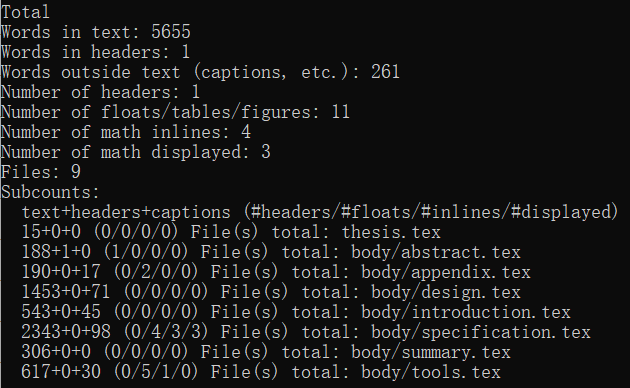
\includegraphics[scale=.5]{figure/texcount.png}  % 选项代表缩小到原图的 0.5 倍。
  \caption{本文字数统计信息}  % 图题
  \label{fig:specification:texcount}  % 定义标签,方便引用该图
\end{figure}

\subsect{pdf 的拆分与合并}
如果最后需要将论文正文、任务书、开题报告、外文译文及原文并入一个 pdf ,可能需要对 pdf 进行拆分与合并。

\LaTeX{} 本身具有合并拆分 pdf 的功能\footnote{使用 pdfpages 宏包。},但是需要自己查文献写代码,相对来说比较麻烦,因此我们可以使用工具对 pdf 进行拆分与合并。

很多浏览器(比如 Edge)和 pdf 阅读器(比如Adobe )应该都具有打印指定页面 pdf 的功能,多次打印不同页面即可达到拆分 pdf 的目的。\hltext{推荐使用谷歌浏览器的打印功能},用谷歌浏览器打开 pdf 就能看到打印按钮了。

\href{https://www.ilovepdf.com/zh-cn/merge_pdf}{ilovepdf 这个网站}可以免费合并多个pdf文件,比较方便。

\subsect{pdf 转 word}
由于学校要求提交 word 稿查重,并且毕业答辩后还要同时提交论文的 word 版和 pdf 版。因此我们使用 \LaTeX{} 编排好精美的pdf论文后,还要将其转成 word 。

好在使用 \LaTeX{} 撰写的 pdf 文件可以\href{https://www.pdfwordconvert.com/zh/convertform}{在这里}轻松转成 word ,并且可以保留几乎所有格式。根据本人亲测的结果,转换后的 word 只存在参考文献引用位置有一点偏差、代码边框展示不全的问题。

转换拆分合并后的 pdf 文件时可能会失败,遇到这种情况时可先将 \LaTeX{} 直接生成的 pdf 文件转成 word ,需要的话再设法合并 word 吧。

打印时使用 pdf 版本即可,甘饴后面的未来图文打印pdf比word每张便宜5分钱(2022年如此,图书馆不清楚)。


\label{chap:模板使用说明:end}

\let\filename\undefined
\let\hltext\undefined
  % 第4章 模板使用说明

% \include{body/detailed_design.tex}

% \newcommand{\nterm}[1]{#1}
\newcommand{\term}[1]{#1}
\newcommand{\filename}[1]{\mbox{\texttt{#1}}}

\chap{系统测试}

BO 编译器的目的是将使用 BO 语言编写的源程序转化为等价的 BOVM 虚拟机能够理解的目标语言程序。如果 BO 编译器存在面对特定输入崩溃、目标代码的行为与源程序语义不一致、错误提示信息有误等问题,可能导致使用 BO 语言的开发人员找不到错误根源,或者用 BO 语言编写的应用程序存在严重问题。因此编译器的可靠性十分关键,我们有必要通过系统化测试找出编译器存在的潜在问题、检验编译器的质量\cite{emark2012}。

\sect{程序运行过程测试}
如图 \ref{fig_test_hello} 所示,\filename{hello.bo} 文件中仅含一条 \verb|println('Hello world!')| 语句。使用 boc 命令产生 \filename{hello.boc} 文件,随后使用 bo 命令执行。BO编译器与BOVM虚拟机运行正常,结果输出 \verb|Hello world!| ,符合预期。
\begin{figure}[H]
    \centering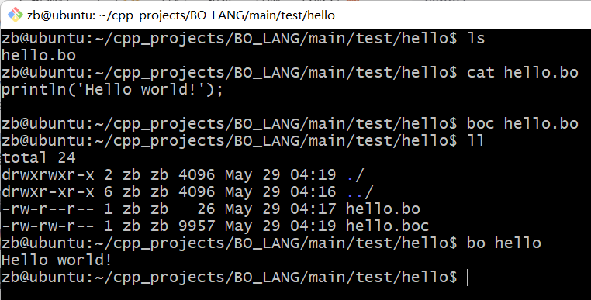
\includegraphics[]{figure/test_hello.pdf}
    \caption{\filename{hello.bo} 文件的编译与运行}
    \label{fig_test_hello}
\end{figure}

\sect{语句测试}

(1) 表达式语句测试

表达式语句的测试用例及运行结果如图 \ref{fig_test_expression} 所示。文件 \filename{expression\_test.bo} 通过直接输出各种表达式的结果进行测试。可见,常量表达式、算术表达式、布尔表达式、以及赋值表达式的结果均符合预期。

\begin{figure}[H]
    \centering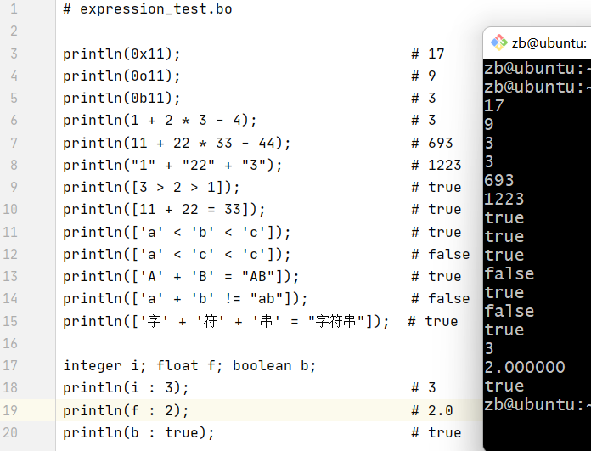
\includegraphics{figure/test_expression.pdf}
    \caption{表达式语句测试}
    \label{fig_test_expression}
\end{figure}


(2) if 语句测试

if 语句的测试用例及运行结果如图 \ref{fig_test_if} 所示。 \verb|if_test| 函数根据形参 a 的值判断它所属的区间,19 到 22 行循环调用函数进行判断,结果符合预期。

\begin{figure}[H]
    \centering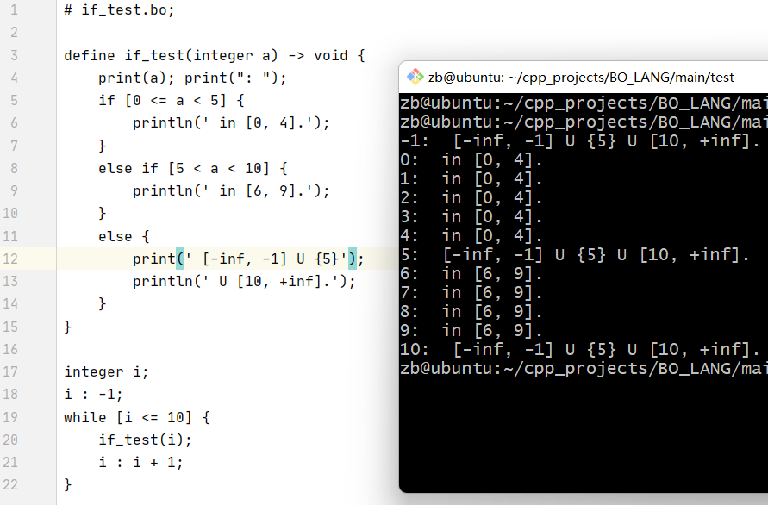
\includegraphics{figure/test_if.pdf}
    \caption{if 语句测试}
    \label{fig_test_if}
\end{figure}

(3) switch 语句测试

switch 语句的测试用例及运行结果如图 \ref{fig_test_switch} 所示。 \verb|switch_test| 函数中的switch语句根据形参 a 的值执行不同的代码块,结果符合预期。

\begin{figure}[H]
    \centering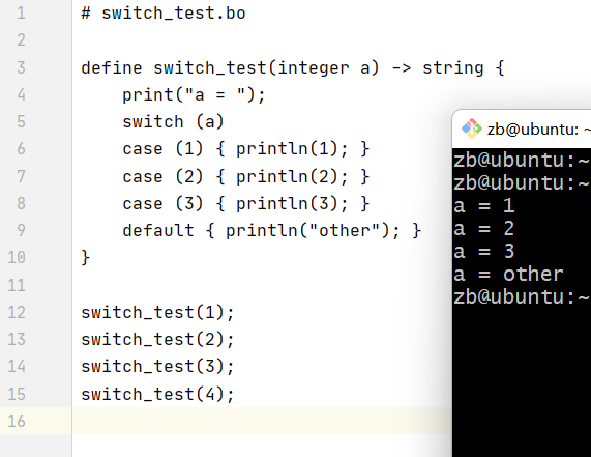
\includegraphics{figure/test_switch.pdf}
    \caption{switch 语句测试}
    \label{fig_test_switch}
\end{figure}

(4) while 语句测试

while 语句的测试用例及运行结果如图 \ref{fig_test_while} 所示。 \verb|isPrime| 函数判断形参 num 是否为素数,第 16 行的 while 语句循环打印数字1到99中的素数,结果符合预期。

\begin{figure}[H]
    \centering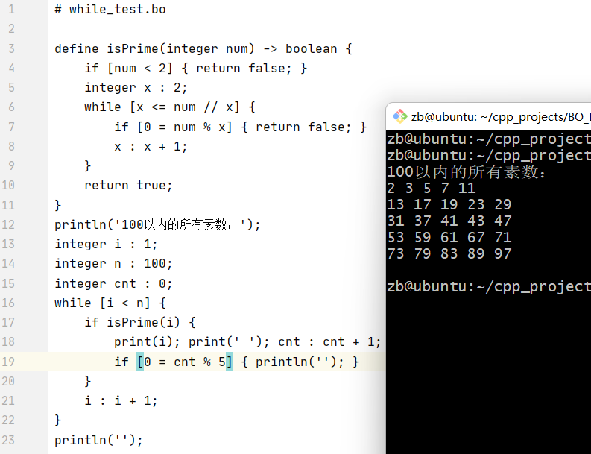
\includegraphics{figure/test_while.pdf}
    \caption{while 语句测试}
    \label{fig_test_while}
\end{figure}

(5) repeat 语句测试

repeat 语句的测试用例及运行结果如图 \ref{fig_test_repeat} 所示。第 8 行的 repeat 语句会执行 end$-$start 次,结果符合预期。

\begin{figure}[H]
    \centering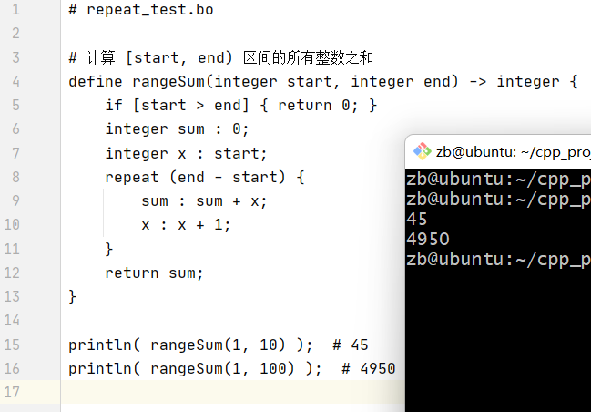
\includegraphics{figure/test_repeat.pdf}
    \caption{repeat 语句测试}
    \label{fig_test_repeat}
\end{figure}

\sect{函数与类的测试}

(1)函数递归测试

函数递归的测试用例及运行结果如图 \ref{fig_test_recur} 所示。 \verb!factorial! 函数递归计算 $n!$ ,结果符合预期。

\begin{figure}[H]
    \centering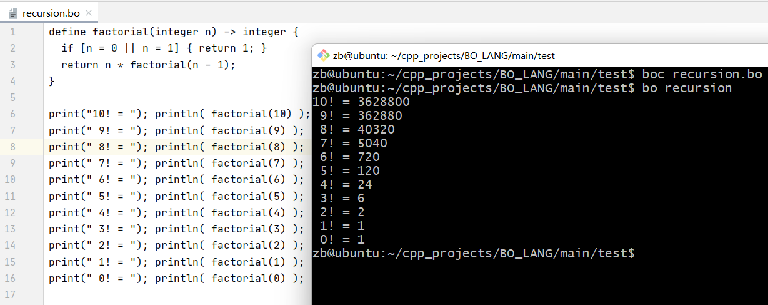
\includegraphics{figure/test_recursion.pdf} 。
    \caption{factorial 函数递归测试}
    \label{fig_test_recur}
\end{figure}

(2)类测试

类测试用例及运行结果如图 \ref{fig_test_class} 所示。 Animal 类被声明为 abstract,代表可被继承,它有一个 type 属性和两个可被覆盖(声明为virtual)的方法,其中 type 代表动物名称、constructor是声明构造方法的关键字; Dog 和 Cat 分别继承了 Animal 类并重写了两个方法。第 19 和 20 行通过父类指针实现多态,运行结果符合预期。

\begin{figure}[H]
    \centering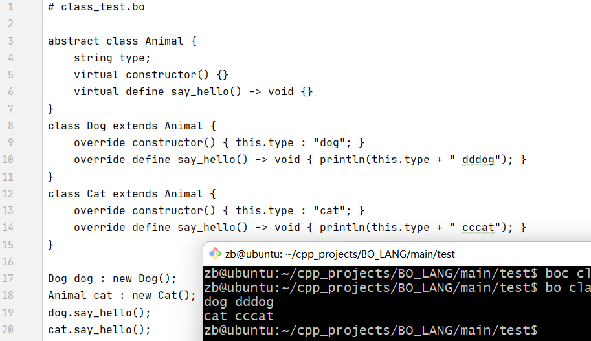
\includegraphics{figure/test_class.pdf}
    \caption{类测试}
    \label{fig_test_class}
\end{figure}

\sect{变量作用域测试}

变量作用域测试用例及运行结果如图 \ref{fig_test_scope} 所示, \filename{test\_scope.bo} 文件中,顶层结构、 if 语句和 func 函数体内各有一个变量 a 的定义。
% 第 2 行变量 a 的作用域是 fun 函数体内,第 7 行变量 a 的作用域是顶层结构,第 11 行的变量 a 的作用域是 if 语句的代码块。
它们的作用域是它们所在的代码块中自身定义位置之后的范围。因此第 10 行的变量 a 定义在第 7 行。测试结果符合预期。
\begin{figure}[H]
    \centering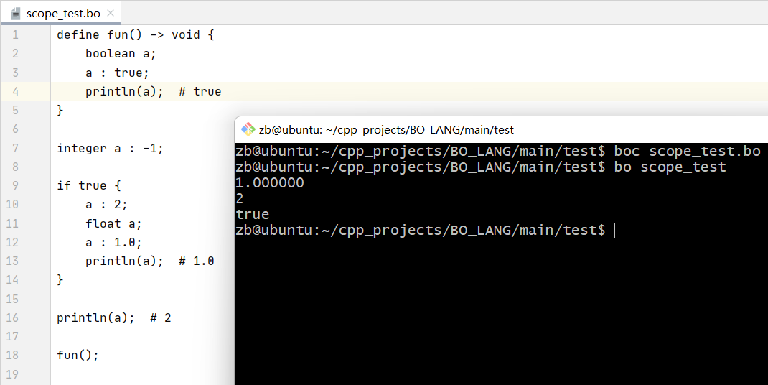
\includegraphics{figure/test_scope.pdf}
    \caption{变量作用域测试}
    \label{fig_test_scope}
\end{figure}

\sect{代码优化测试}

代码优化效果无法直接从 BO 编译器的运行结果观察,因此我们采用 bop 命令可视化查看编译生成的 \filename{.boc} 文件中的字节码。真正的字节码仅由二进制的 0 和 1 组成, bop 命令会将其解析为助忆符的形式展现。

(1)表达式语句代码优化测试

表达式语句代码优化测试用例及运行结果如图 \ref{test_optimizer1} 所示。表达式 $1+2*3-\text{t}$ 折叠成为 $7-\text{t}$ ,表达式 $\text{t}+2*3-4$ 折叠成为 $\text{t}+6-4$ 。测试结果符合预期。

\begin{figure}[H]
\centering
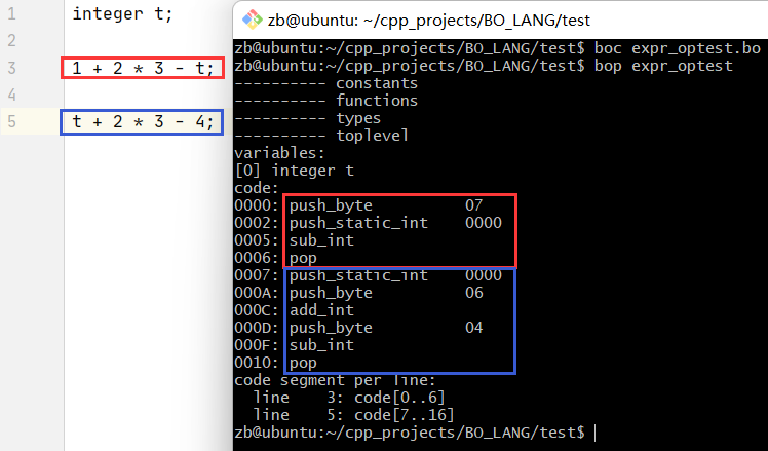
\includegraphics{figure/test_optimizer1.pdf}
\caption{表达式语句代码优化测试}
\label{test_optimizer1}
\end{figure}

(2)if 语句代码优化测试

if 语句代码优化测试用例及运行结果如图 \ref{test_optimizer2} 所示。条件为true的if块被展开,条件为false的if块被消去。测试结果符合预期。

\begin{figure}[H]
\centering
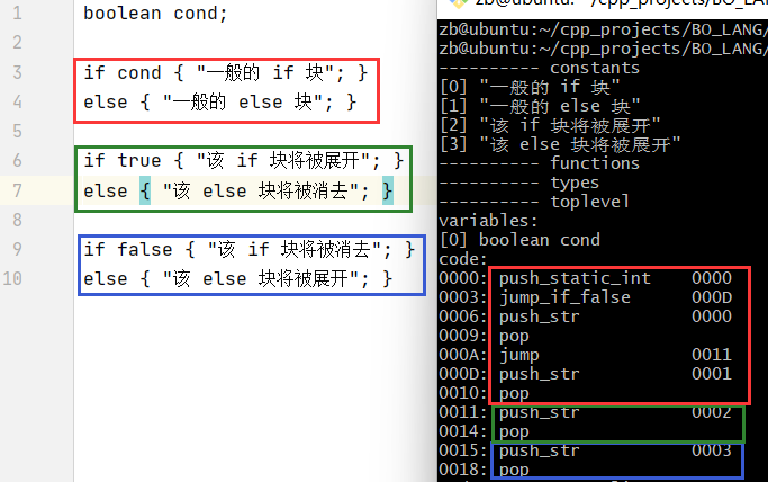
\includegraphics{figure/test_optimizer2.pdf}
\caption{if 语句代码优化测试}
\label{test_optimizer2}
\end{figure}

(2)while 语句代码优化测试

while 语句代码优化测试用例及运行结果如图 \ref{test_optimizer3} 所示。break语句之后的字节码被消去。测试结果符合预期。

\begin{figure}[H]
\centering
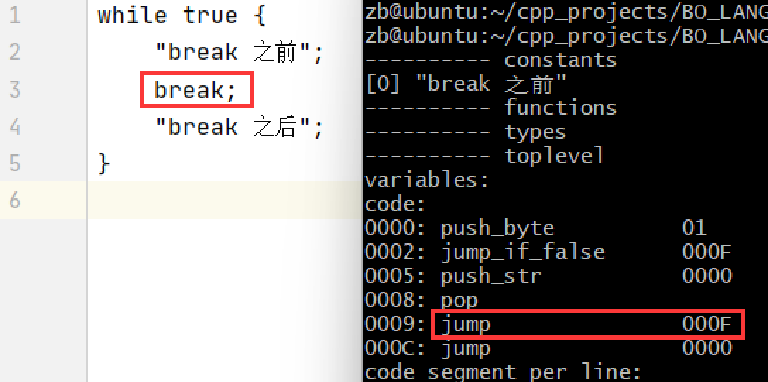
\includegraphics{figure/test_optimizer3.pdf}
\caption{while 语句代码优化测试}
\label{test_optimizer3}
\end{figure}

(2)repeat 语句代码优化测试

repeat 语句代码优化测试用例及运行结果如图 \ref{test_optimizer4} 所示。循环 0 次的代码块直接消去,循环 1 次的代码块直接展开。测试结果符合预期。

\begin{figure}[H]
\centering
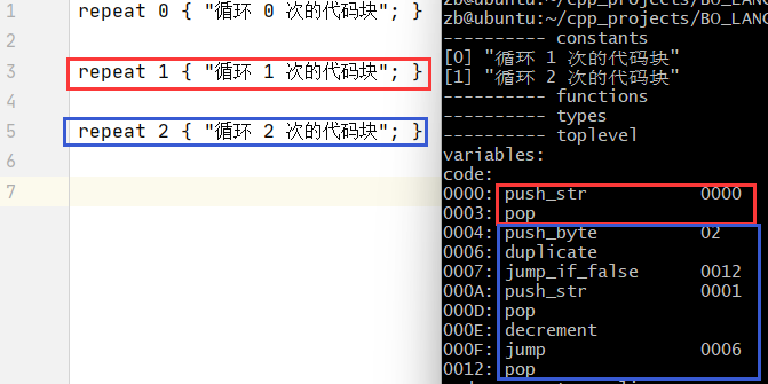
\includegraphics{figure/test_optimizer4.pdf}
\caption{repeat 语句代码优化测试}
\label{test_optimizer4}
\end{figure}

\sect{错误处理测试}

 BO 编译器一旦发现语法或语义错误便会立即报告当前错误并终止,因此我们只需构造存在一条错误语句的程序进行测试即可。

(1)词法错误处理测试

词法错误处理测试用例及运行结果如图 \ref{fig_test_scanner_error} 所示,编译器指出在 \filename{scanner\_error\_test.bo} 文件的第 10 行 7 列在非注释环境下出现了一个非法字符 \verb!@! 。由于此时尚未进行语义分析,所以编译器尚未发现第 3 行存在未定义标识符,运行结果符合预期。

\begin{figure}[H]
    \centering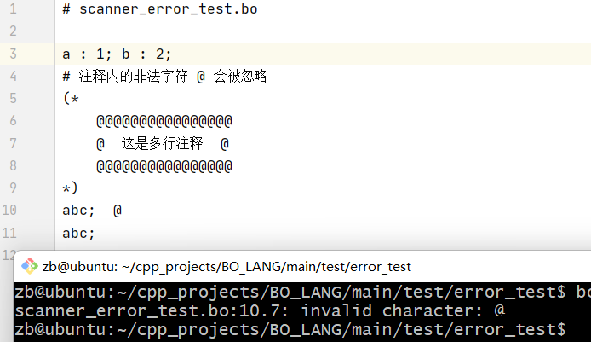
\includegraphics[width=13cm]{figure/test_scanner_error.pdf}
    \caption{词法错误处理测试}
    \label{fig_test_scanner_error}
\end{figure}

(2)语法错误处理测试

语法错误处理测试用例及运行结果如图 \ref{fig_test_parser_error} 所示,编译器指出在第 5 行 1 列识别到了一个非预期的标识符,并表示预期读入一个分号。由于此时尚未进行语义分析,所以编译器尚未发现第 3 行存在未定义标识符,运行结果符合预期。

\begin{figure}[H]
    \centering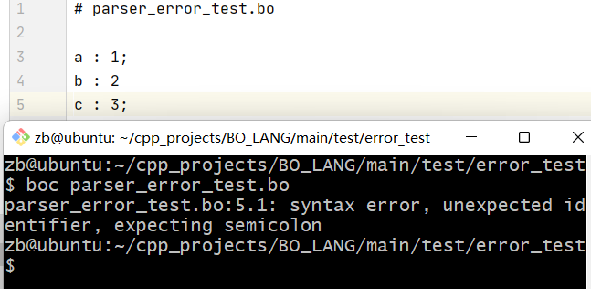
\includegraphics[width=13cm]{figure/test_parser_error.pdf}
    \caption{语法错误处理测试}
    \label{fig_test_parser_error}
\end{figure}

(3)语义错误处理测试

语义错误处理测试用例及运行结果如图 \ref{fig_test_semantic_error} 所示,编译器指出在第 10 行类成员 b 不可访问,结果符合预期。

\begin{figure}[H]
    \centering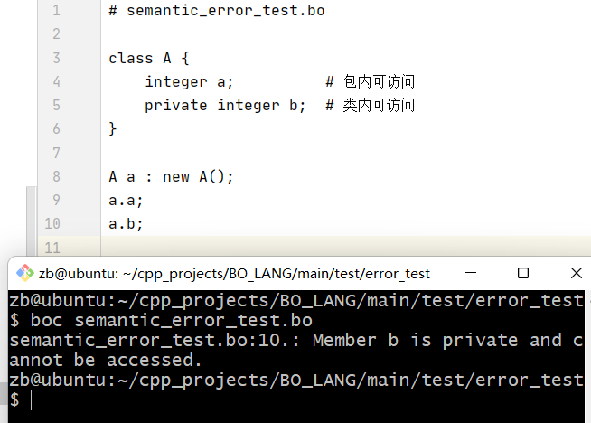
\includegraphics[width=13cm]{figure/test_semantic_error.pdf}
    \caption{语义错误处理测试}
    \label{fig_test_semantic_error}
\end{figure}


% \sect{性能测试}







\let\nterm\undefined
\let\term\undefined
\let\filename\undefined







% 假设已存在定义 \verb!integer i;! \verb!float f;! \verb!boolean b;! \verb!string s;! 。对表达式语句的测试如表 \ref{tab_test_expr} 所示。
% \newcommand{\widthOfRes}{4cm}
% \begin{table}[H]
% \centering
% \caption{表达式语句测试用例}
% \begin{tabular}[]{@{}lllll@{}}
%     \toprule
%     类型         & 表达式                         & 预期结果      & 实际结果   &  是否通过                       \\
%     \midrule
%     十六进制整型    &  \verb!0x11!                &  17           & 17                           &   通过                    \\
%     八进制整型      &  \verb!0o11!                &  9            & 9                            &   通过                    \\
%     二进制整型      &  \verb!0b11!                &  3            & 3                            &   通过                    \\
%     算术表达式      &  \verb!11 + 22 * 33 - 44!   &  693          & 693                          &   通过                    \\
%     布尔表达式      &  \verb![3 > 2 > 1]!         &  true         & true                         &   通过                    \\
%     布尔表达式      &  \verb!['a' < 'b' < 'c']!   &  true         & true                         &   通过                    \\
%     布尔表达式      &  \verb!['a' < 'd' < 'c']!   &  false        & false                        &   通过                    \\
%     布尔表达式      &  \verb!['A' + 'B' = "AB"]!  &  true         & true                         &   通过                    \\
%     非法表达式      &  \verb!i = 1!               & 语法错误       & \parbox[t]{\widthOfRes}{unexpected token: =}  &   通过                    \\
%     赋值表达式      &  \verb!i : 1!               & 1             & 1  &   通过                    \\ 
%     赋值表达式      &  \verb!i : s!               & 语义错误       & \parbox[t]{\widthOfRes}{Cannot cast from string to integer.}  &   通过                    \\ 
%     赋值表达式      &  \verb!f : 2!               & 2.000000       & 2.000000  &   通过                    \\ 
%     加法表达式      &  \verb!i + b!               & 语义错误       & \parbox[t]{\widthOfRes}{The operand type of the arithmetic operator is invalid.}  &   通过                    \\ 
%     非法表达式      &  \verb!@abc!               & 词法错误       & \parbox[t]{\widthOfRes}{invalid character: @}  &   通过                    \\
%     \bottomrule
% \end{tabular}
% \label{tab_test_expr}
% \end{table}
% \let\widthOfRes\undefined


%%%%%%%%%%%%%%%%%%%%%%%%%%%%%%%%%%%%%%%%%%%%%%%%%%%%%%%%%%%%%%%%%%%%%%%
%%%%%%%%%%%%%%%%%%%%%%%%%%%%%%%%%%%%%%%%%%%%%%%%%%%%%%%%%%%%%%%%%%%%%%%
%%%%%%%%%%%%%%%%%%%%%%%%%%%%%%%%%%%%%%%%%%%%%%%%%%%%%%%%%%%%%%%%%%%%%%%
%%%%%%%%%%%%%%%%%%%%%%%%%%%%%%%%%%%%%%%%%%%%%%%%%%%%%%%%%%%%%%%%%%%%%%%
%%%%%%%%%%%%%%%%%%%%%%%%%%%%%%%%%%%%%%%%%%%%%%%%%%%%%%%%%%%%%%%%%%%%%%%
%%%%%%%%%%%%%%%%%%%%%%%%%%%%%%%%%%%%%%%%%%%%%%%%%%%%%%%%%%%%%%%%%%%%%%%


% 假设已存在如图 \ref{fig_class_def} 所示类 Animal、Dog、Cat、Person 以及相关变量的定义。对类的封装、继承和多态的测试如表 \ref{tab_test_class} 所示。
% 
% \begin{figure}[H]
% \centering
% \begin{subfigure}[b]{.45\textwidth}
% \vspace{0pt}
% \centering
% \begin{lstlisting}[numbers=none]
% abstract class Animal {
%     virtual define sayHello() -> void {}
% }
% class Dog extends Animal {
%     override sayHello() -> void {
%         println("dog hello");
%     }
% }
% class Cat extends Animal {
%     override sayHello() -> void {
%         println("cat hello");
%     }
% }
% \end{lstlisting}
% \caption{类 Animal 及其子类的定义}
% % \label{fig_func_call_expr_2}
% \end{subfigure}
% \quad\quad
% \begin{subfigure}[b]{.45\textwidth}
% \vspace{0pt}
% \centering
% \begin{lstlisting}[numbers=none]
% class Person {
%     public string name;
%     private integer age;
%     define constructor
%     initialize(string name, integer age) {
%         this.name : name;
%         this.age : age;
%     }
% }
% Person p1 : new Person("Bob", 22);
% Person p2;
% Animal dog : new Dog();
% Animal cat : new Cat();
% \end{lstlisting}
% \caption{类 Object 与变量的定义}
% % \label{fig_func_call_expr_2}
% \end{subfigure}
% \caption{待测试类的定义}
% \label{fig_class_def}
% \end{figure}

% \newcommand{\widthOfRes}{4cm}
% \begin{table}[H]
% \centering
% \caption{流程控制语句测试用例}
% \begin{tabular}[]{@{}lllll@{}}
%     \toprule
%     类型           & 表达式           & 预期结果      & 实际结果   &  是否通过                       \\
%     \midrule
%     类成员访问表达式  &  p1.name         &  Bob           & Bob                          &   通过                    \\
%     类成员访问表达式  &  p1.age          &  语法错误       & Member age is private.       &   通过                    \\
%     类成员访问表达式  &  p2.name         &  空指针异常     & Exception occured: null pointer.     &   通过                    \\
%     类成员访问表达式  &  dog.sayHello()  &  dog hello     & dog hello                          &   通过                    \\
%     类成员访问表达式  &  cat.sayHello()  &  cat hello     & cat hello                         &   通过                    \\
%     \bottomrule
% \end{tabular}
% \label{tab_test_class}
% \end{table}
% \let\widthOfRes\undefined

% \FloatBarrier

% \FloatBarrier


% \sect{功能测试}
% \subsec{表达式语句测试}

% \subsec{流程控制语句测试}
% 假设已存在如图 \ref{fig_func_def} 所示 getGrade 与 rangeSum 的函数定义。对流程控制语句的测试如表 \ref{tab_test_con} 所示。


% \begin{figure}[H]
% \centering
% \begin{subfigure}[b]{.45\textwidth}
% \vspace{0pt}
% \centering
% \begin{lstlisting}[numbers=none]
% # 根据分数判断等级
% define getGrade(integer score) -> string {
%     string grade : null;
%     if [score >= 90] { grade : 'A'; }
%     else if [score >= 80] { grade : 'B'; }
%     else if [score >= 60] { grade : 'C'; }
%     else { grade : 'D'; }
%     return grade;
% }
% \end{lstlisting}
% \caption{getGrade 函数定义}
% % \label{fig_func_call_expr_2}
% \end{subfigure}
% \quad
% \begin{subfigure}[b]{.5\textwidth}
% \vspace{0pt}
% \centering
% \begin{lstlisting}[numbers=none]
% # 计算 [start, end) 区间的所有整数之和
% define rangeSum(integer start, integer end) 
%     -> integer {
%     if [start > end] { return 0; }
%     integer sum : 0;
%     integer x : start;
%     while [x != end] {
%         sum : sum + x;
%         x : x + 1;
%     }
%     return sum;
% }
% \end{lstlisting}
% \caption{rangeSum 函数定义}
% % \label{fig_func_call_expr_2}
% \end{subfigure}
% \caption{待测试函数定义}
% \label{fig_func_def}
% \end{figure}

% \newcommand{\widthOfRes}{4cm}
% \begin{table}[H]
% \centering
% \caption{流程控制语句测试用例}
% \begin{tabular}[]{@{}lllll@{}}
%     \toprule
%     类型         & 表达式或语句                         & 预期结果      & 实际结果   &  是否通过                       \\
%     \midrule
%     函数调用表达式  &  getGrade(95)  &  A           & A                           &   通过                    \\
%     函数调用表达式  &  getGrade(85)  &  B            & B                            &   通过                    \\
%     函数调用表达式  &  getGrade(75)  &  C            & C                            &   通过                    \\
%     函数调用表达式  &  getGrade(60)  &  C          & C                          &   通过                    \\
%     函数调用表达式  &  getGrade(59)  &  D         & D                         &   通过                    \\
%     函数调用表达式  &  getGrade(45)  &  D         & D                         &   通过                    \\
%     函数调用表达式  &  rangeSum(1, 10)  &  45         & 45                         &   通过                    \\
%     函数调用表达式  &  rangeSum(1, 100)  &  4950         & 4950                         &   通过                    \\
%     非法 if 语句        &  if (true) ;   & 语法错误    & unexpected ;, expecting \verb!{!   & 通过  \\
%     if 语句        &  if (true) {}   & 正常运行    & 正常运行   & 通过  \\
%     非法 if 语句        &  if (1) {}   & 语义错误    & \parbox[t]{\widthOfRes}{The conditional expression must be a boolean type.}   & 通过  \\
%     \bottomrule
% \end{tabular}
% \label{tab_test_con}
% \end{table}
% \let\widthOfRes\undefined


\chap{总结与展望}

\sect{213}

\thesection

\section*{111}
\thesection

\sect{111.1}

\sect{111.2}

\section{222}
\thesection

%% 参考文献开始一级标题不编号
% \ctexset{section/numbering=false}
\setcounter{secnumdepth}{0}
%%

\chap{参考文献}

\nocite{*}
\printbibliography[heading=none]

\chap{致谢}

\appendix  % 附录开始

\chap{附录撰写示例}  % 附录 A
\sect{附录的二级标题实例}
本模板不会将附录的二级标题加入目录,如有需要,请自行实现。
\subsect{附录的三级标题实例}
本模板不会将附录的三级标题加入目录,如有需要,请自行实现。
\sect{附录图表示例}

长沙理工大学校徽如图 \ref{fig:appendix:csustlogo} 所示。  % 使用 \ref 命令引用图片标签

\begin{figure}[htbp]  % htbp选项允许浮动体出现在任意位置,后文详述
  \centering  % 表格居中
  
\includegraphics[scale=.5]{figure/csustlogo_626by572.jpg}  % 选项代表缩小到原图的 0.5 倍。
  \caption{长沙理工大学校徽}  % 图题
  \label{fig:appendix:csustlogo}  % 定义标签,方便引用该图
\end{figure}

浮动体选项及其含义如表 \ref{tab:appendix:floatchoice} 所示。

\begin{table}[htbp]
  \centering  % 表格居中
  \zihao{5}  % 五号字体
  \caption{浮动体选项及其含义}
  % \vspace{-3mm}
  \begin{tabular}[]{ll}
      \toprule   % 三线表的第一条线
      表项      & 含义            \\
      \midrule   % 三线表的第二条线
        !       &  忽略一些严格的限制   \\
        h       &  如果可以,放在当前位置   \\
        t       &  允许放在顶部   \\
        b       &  允许放在底部  \\
        p       &  运行放在浮动栏或浮动页   \\
        H       &  禁止浮动   \\
      \bottomrule   % 三线表的第三条线
  \end{tabular}
  \label{tab:appendix:floatchoice}  % 注意:这不是伪代码
\end{table}


\chap{文档类 csustThesis 完整代码}  % 附录 B
\sect{标题1}
\subsect{标题11}
\sect{标题2}
\subsect{标题21}


\chap{插图与表格汇总}  % 附录 C

\listoffigures

\listoftables

\end{document}

